\documentclass[a4paper]{article}

\usepackage[english]{babel}
\usepackage[utf8x]{inputenc}
\usepackage{amsmath}
\usepackage{mathtools}
\usepackage{graphicx}
\usepackage{listings}
\usepackage{float}
\usepackage[colorinlistoftodos]{todonotes}

\DeclarePairedDelimiter\ceil{\lceil}{\rceil}
\DeclarePairedDelimiter\floor{\lfloor}{\rfloor}

\title{HW3 (resubmitted)}
\author{Matthew Flickner, Jeff Fennell, Joseph Barbosa, Misa Pham}

\begin{document}


\maketitle

\section*{1}

 \lstinputlisting[language=Python]{bozosort.py}
 
\begin{table}[h]
\begin{tabular}{ccccccc}
List Size              & Test 1                     & Test 2                     & Test 3                    & Test 4                     & Test 5                     & Average                      \\ \cline{2-7} 
\multicolumn{1}{c|}{2} & \multicolumn{1}{c|}{3}     & \multicolumn{1}{c|}{1}     & \multicolumn{1}{c|}{2}    & \multicolumn{1}{c|}{5}     & \multicolumn{1}{c|}{5}     & \multicolumn{1}{c|}{3.2}     \\ \cline{2-7} 
\multicolumn{1}{c|}{3} & \multicolumn{1}{c|}{9}     & \multicolumn{1}{c|}{8}     & \multicolumn{1}{c|}{21}   & \multicolumn{1}{c|}{7}     & \multicolumn{1}{c|}{8}     & \multicolumn{1}{c|}{10.6}    \\ \cline{2-7} 
\multicolumn{1}{c|}{4} & \multicolumn{1}{c|}{66}    & \multicolumn{1}{c|}{3}     & \multicolumn{1}{c|}{12}   & \multicolumn{1}{c|}{18}    & \multicolumn{1}{c|}{34}    & \multicolumn{1}{c|}{26.6}    \\ \cline{2-7} 
\multicolumn{1}{c|}{5} & \multicolumn{1}{c|}{21}    & \multicolumn{1}{c|}{7}     & \multicolumn{1}{c|}{132}  & \multicolumn{1}{c|}{53}    & \multicolumn{1}{c|}{46}    & \multicolumn{1}{c|}{51.8}    \\ \cline{2-7} 
\multicolumn{1}{c|}{6} & \multicolumn{1}{c|}{619}   & \multicolumn{1}{c|}{1834}  & \multicolumn{1}{c|}{2484} & \multicolumn{1}{c|}{2640}  & \multicolumn{1}{c|}{800}   & \multicolumn{1}{c|}{1675.4}  \\ \cline{2-7} 
\multicolumn{1}{c|}{7} & \multicolumn{1}{c|}{569}   & \multicolumn{1}{c|}{11549} & \multicolumn{1}{c|}{6883} & \multicolumn{1}{c|}{7143}  & \multicolumn{1}{c|}{3203}  & \multicolumn{1}{c|}{5869.4}  \\ \cline{2-7} 
\multicolumn{1}{c|}{8} & \multicolumn{1}{c|}{26807} & \multicolumn{1}{c|}{8656}  & \multicolumn{1}{c|}{3150} & \multicolumn{1}{c|}{14815} & \multicolumn{1}{c|}{50008} & \multicolumn{1}{c|}{20687.2} \\ \cline{2-7} 
\end{tabular}
\end{table}

\section*{2}

\lstinputlisting[language=Java]{ViginereCypher.java}

Code output:

plaintext: attackatdawn
keyword: hello
cypherText: hxelqktmdcgn

plaintext: hellomynameisjeff
keyword: agoodkey
cypherText: hkzzrwclhqptgvcsf

plaintext: mamailoveyou
keyword: gains
cypherText: saunaxohegzi

plaintext: yolo
keyword: hi
cypherText: fwjc


\section*{3}
The frequency of each letter is as follows:

A: 6, 3.10\%\newline
B: 4, 2.08\%\newline
C: 0, 0.00\%\newline
D: 9, 4.69\%\newline
E: 8, 4.17\%\newline
F: 4, 2.08\%\newline
G: 0, 0.00\%\newline
H: 6, 3.125\%\newline
I: 14, 7.29\%\newline
J: 1, 0.52\%\newline
K: 5, 2.60\%\newline
L: 10, 5.21\%\newline
M: 14, 7.29\%\newline
N: 0, 0.00\%\newline
O: 19, 9.90\%\newline
P: 1, 0.52\%\newline
Q: 29, 15.10\%\newline
R: 17, 8.85\%\newline
S: 1, 0.52\%\newline
T: 12, 6.25\%\newline
U: 4, 2.08\%\newline
V: 7, 3.65\%\newline
W: 19, 9.90\%\newline
X: 2, 1.04\%\newline
Y: 0, 0.00\%\newline
Z: 0, 0.00\%\newline

The decrypted text (with spaces \& punctuation added) is:

\textbf{\textit{Let us change our traditional attitude to the construction of programs. Instead of imagining that our main task is to instruct a computer what to do, let us concentrate rather on explaining to human beings what we want a computer to do.}}

\section*{4}
This was in the original HW but appear in the wrong section of the document so we received a zero on the question.
\begin{figure}[H]
\centering
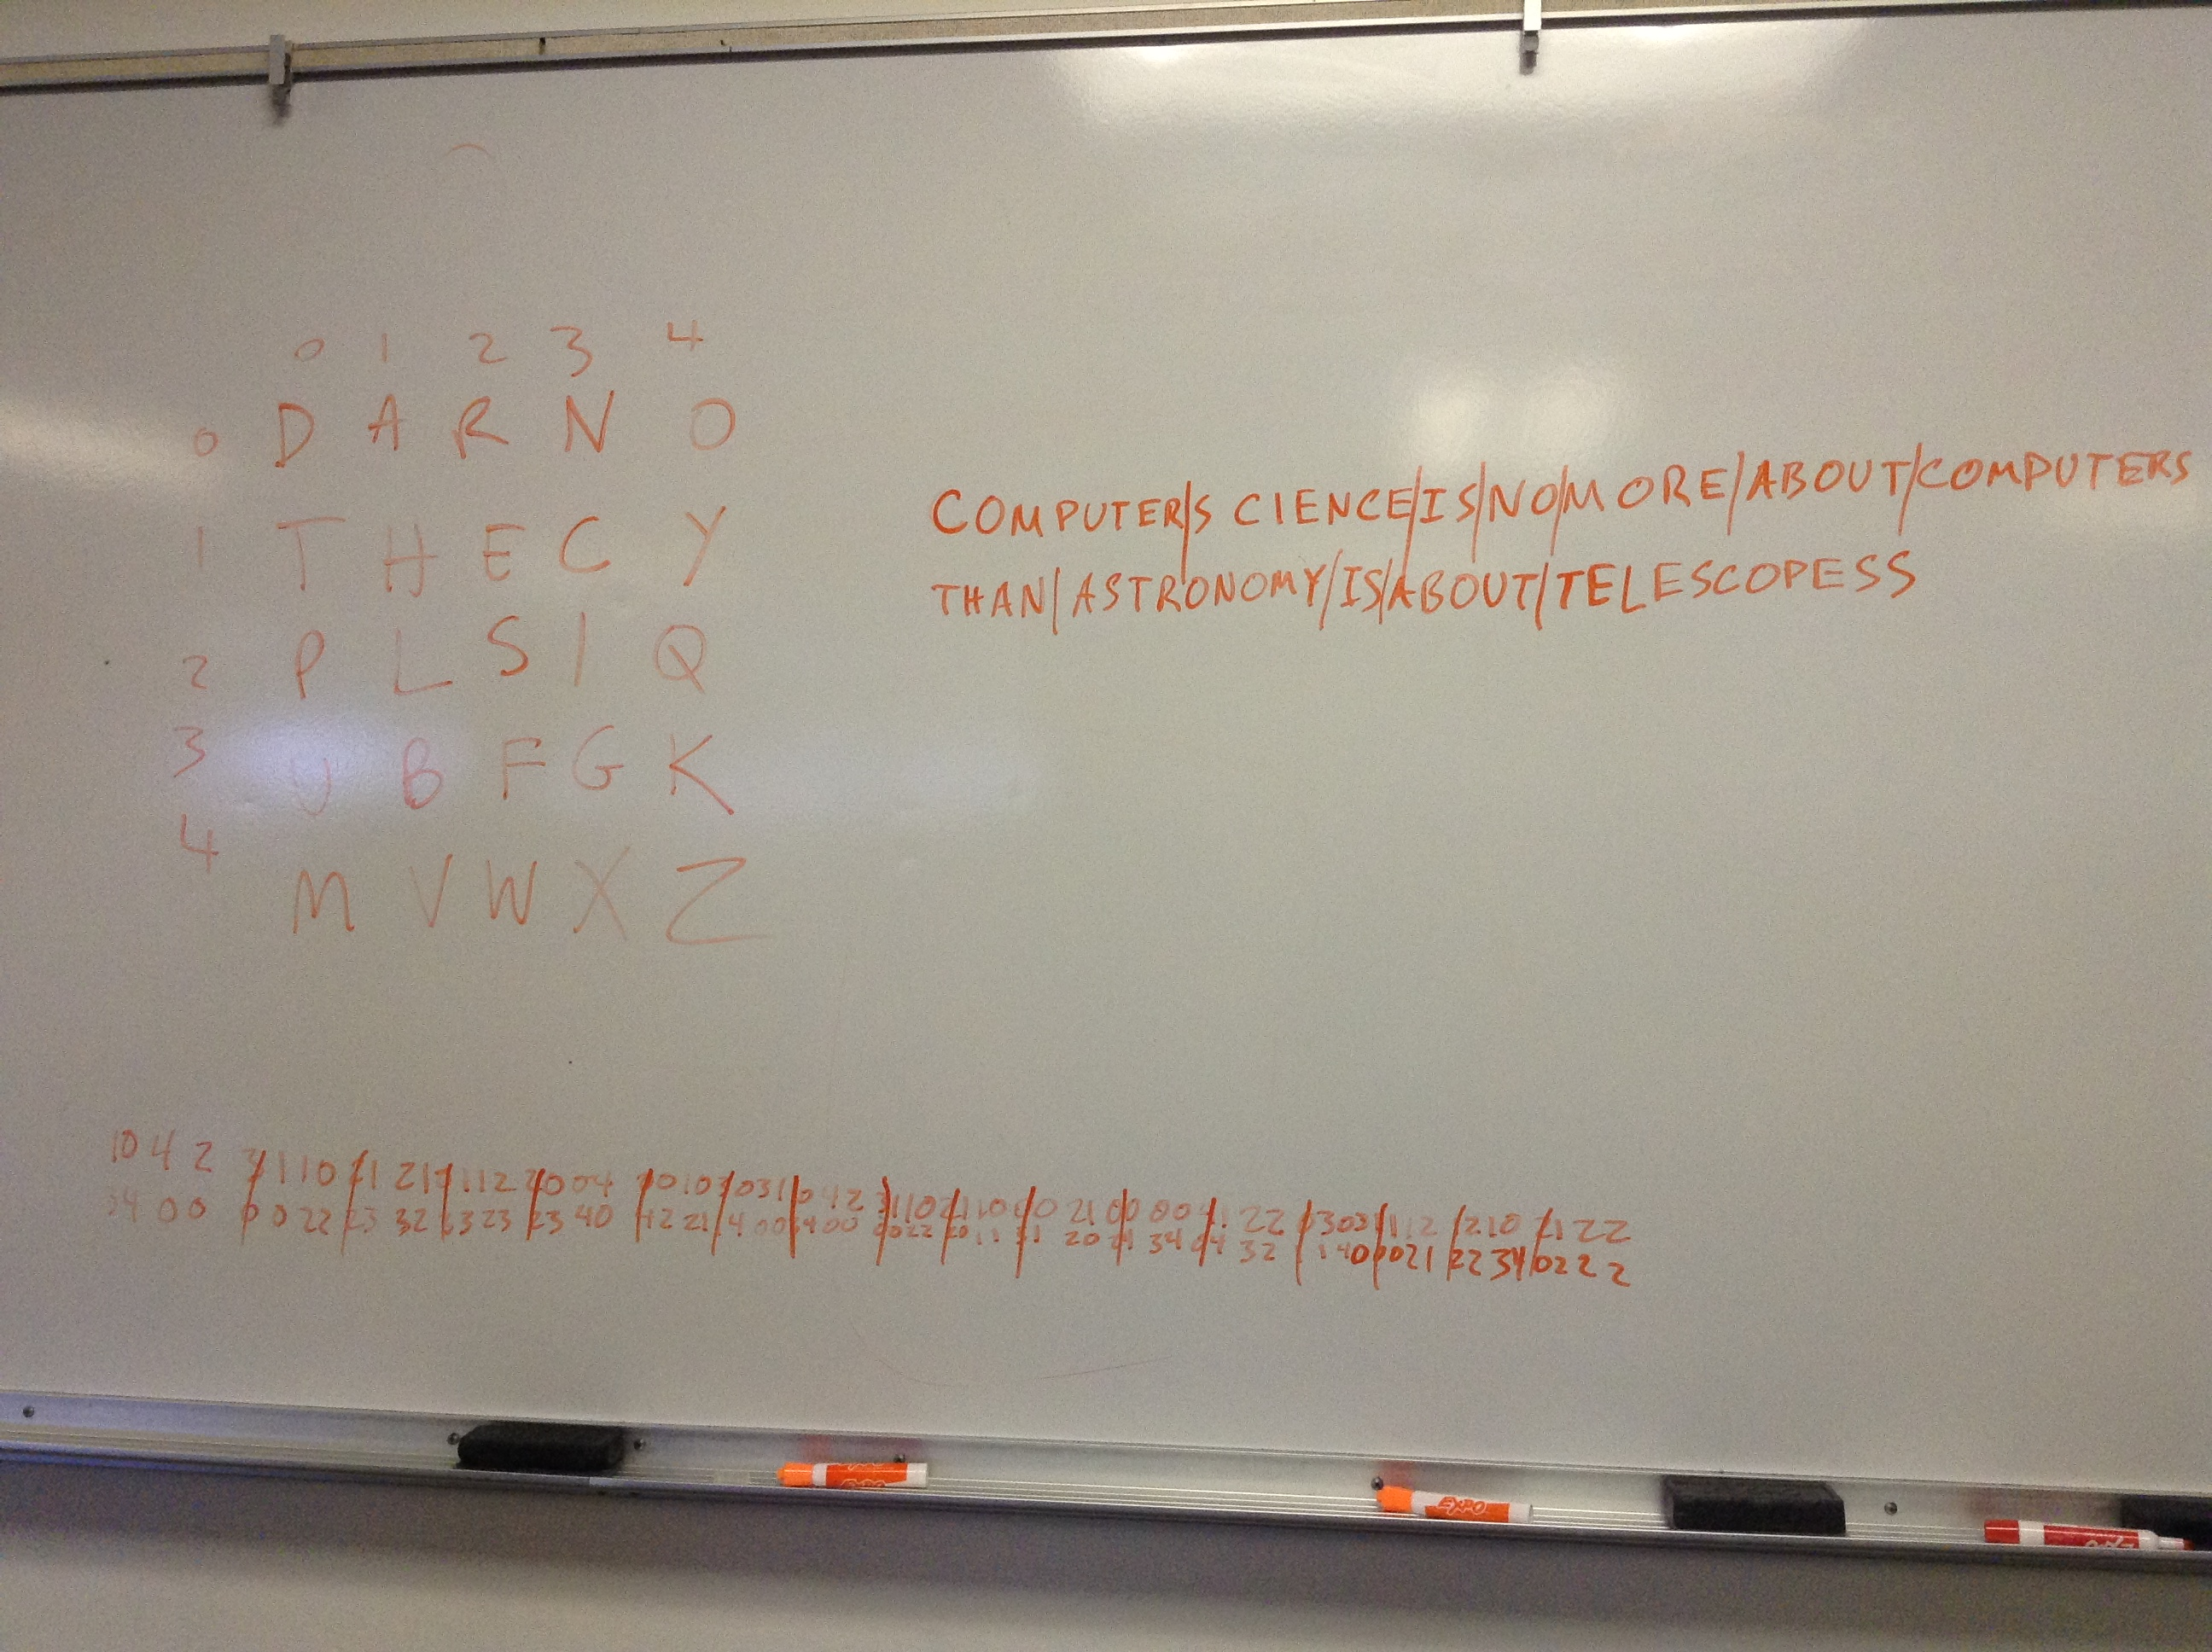
\includegraphics[width=0.8\textwidth]{prob4.jpg}
\end{figure}

\section*{5}

Given that somebodies RSA public key is (729880581317, 5), given in notation (N, e) where we know that N = p * q, we can solve for their private key. In order to do so we must first calculate what p and q are; since they both must be prime we should be able to prime factor our N and get a result. After prime factorization of 729880581317 I found the result to be 822893 * 886969. After doing so, we can then take (p-1) and (q-1), which would be 822892 and 886968, we multiply these to test if our e is relatively prime to the result. That is, we must test if our result and our given e have a greatest common factor of 1, which after testing so we discover that they do. Since the result, 729878871456, checks out we can use it to determine our private key, d. To find the private key, we need to calculate the modular inverse of our e, 5, relative to 729878871456. 
\\
\\
By using the Euclidean algorithm to find the greatest common divisor until we get a remainder of 1, the steps are as follows: 
\\
\\
729878871456 = 5 * 145975774291 + 1
\\
after 1 step we hit a remainder of 1 so we need to simplify backwards now and we get
\\
1 = 729878871456 + 5 * (-145975774291)     (since we want our original two values to be positive)
\\
making our inverse mod value equal to -145975774291 which in mod 729878871456 turns out to be 583903097165. If we multiply this value by our e, 5, and mod it by our value of 729878871456 we get a result of 1, further proving our answer to be the inverse mod. 
\\

\section*{6) 1.45}
a Digitial signature ensures that messages being received are coming from the original sender and not from a malicious sender. Drawing from the class example, signatures ensure that Bob is receiving messages from Alice and not messages from Mal.

b) An RSA signature consists of sign(M, d) = Md(mod N), where d is a secret key and N is part of the public key. Show that anyone who knows the public key (N, e) can perform verify((N, e), $M^{d}, M)$, i.e., they can check that a signature really was created by the private key. Give an implementation and prove its correctness.

Suppose we have two private keys, The relationship between the public and private key is as follows:
$M =  \sigma^{e} mod N$. 

Therefore, all the receiver needs to do is solve this modular arithmetic to verify that the private key was sent. 

Verify takes in a public key (N, e), a signature $\sigma$, and a message M as its parameters. The signature, $\sigma$, is created by the sign procedure which takes in a message M and a secret key to generate $M^{d}(mod N)$. Anyone with the public key can perform the verify procedure because the signature is given and a component of the signature is M. Therefore all the parameters of the verify procedure are filled. Taking in the public key, signature, and message, the verify procedure can be executed to make sure that the signature was created by the private key. An implementation of this is Alice signing her message before sending it to Bob by passing in her secret key and message to create her signature. 

c) I picked $p = 137, q = 71$. Hence $N = pq = 9727$ and $(p−1)(q −1) = 9520 = 2^4 * 5 * 7 * 17$. Then, I chose $e = 99$, which is coprime to 9520. d must then be the inverse of e mod 9520, that is 6539, found by running Extended Euclid. Using the letter L, we can use it's binary representation in which it equals 76. Then, the signature of this first number is $76^99 mod 9727 = 4814$. Finally, $4814^99 mod 9727 = 76$, as required.

d) 391 can be factored as $17 · 23$. Then $16 * 22 = 352$. Thus $d = (e)^−1 mod 352 = 145$. Actually, $145 * 17 = 2465 = 1 mod 352$.

\section*{7) 1.46}

a) If Bob agrees to sign anything that he is asked to, Alice could send out a message to Bob and Eve could have Bob sign it the message which would just decrypt the message.

b) e and N are public. So if Eve intercepts the message from Alice she can find a value that is co-prime to the public N and mod it with the number to the e. After she has that if she gets Bob's signature she can do a computation similar to what we did in problem 5 for the inverse mod of the value she previously found using the public key, this gives her the answer if she mods it then multiplies with her message.

\section*{8) 2.4}
We can use Master Theorem here.\\
\\
For Algorithm A:\\
$T(n) = 5T(n/2) + n$ where
$a=5, b=2, d=1$.\\
Since $log_2 (5) > 1$, Algorithm A is $\Theta(n^{log_2(5)})$.
\\
\\
For Algorithm B:\\
We cannot use Master Theorem for B. Algorithm B is $O(2^{n-1})$ as far as efficiency goes because each recursion is two subproblems of size $(n-1)$. Combination in constant time $O(1)$ would make $B = O(2^{n-1})$. Doing some math, $B = O(1/2*2{n})$ which is just $\Theta(2^{n})$.
\\
\\
For Algorithm C:\\
$T(n) = 9T(n/3) + n^2$ where
$a=9, b=3, d=2$.\\
Since $log_3(9) = 2$, by Master Theorem, Algorithm C is $\Theta(n^{2}logn)$.
\\
\\
I would choose Algorithm A because it is the most efficient as far as its asymptotics go. B is the least efficient despite its constant time combination. Although 3 is partially logarithmic, it is also quadratic which greatly diminishes its efficiency. Initially, C appears to be more efficient but at large values of n, A is the best bet.



\section*{9) 2.12}
By the Master Theorem,
$T(n) = 2(n/2) + 1$ where
$a=2, b=2, d=0$.
Since $log_2(2) > 0$, there are $\Theta(n^{log_2(2)})$ prints which simplifies to $\Theta(n^{1})$ or just $\Theta(n)$.


\section*{10) 2.23}

a) 

Given an array, a, of n elements of type T.
\begin{verbatim}
GetMajority(a[1...n]) {
	
	if n = 1 {
		return a[1]
	}

	half = Math.floor(n/2)
	majority1 = GetMajorityElement(a[1...half])
	majority2 = GetMajorityElement(a[half+1...n]

	if (majority1 = majority2) {
		return majority1;
	}

	count1 = GetFrequency(a[1...n],majority1)
	count2 = GetFrequency(a[1...n],majority2)

	if count1 > half+1 {

		return count1

	} else if rcount > k+1: {
		
		return count2

	} else {

		return no majority element

	}
\end{verbatim}


b) 
Given an array, a, of n elements of type T\\
Create a Hashtable (T, int) Totals
\begin{verbatim}
//Count the number of times each element appears
For each a[0...n] {
	int total = Totals.get(a[i])
	total +=1
	Totals.put(a[i], total)
}
	mostOccurring = a[0]

//Find the element that occurs the most\\
For each a[1...n] {
	if Totals.get(a[i]) > Totals.get(mostOccurring) {
		a[i] = Totals.get(mostOccurring)
	}
}

//Check to see if element that occurs the most is the majority element
if Total.get(mostOccurring) >= (n/2) {
	
	return mostOccurring;
} else {
	
	print ``no majority exists''
}
\end{verbatim}
open 

\section*{11) 3.2(a)}
A $\rightarrow$ B $\rightarrow$ C $\rightarrow$ D $\rightarrow$ H $\rightarrow$ G $\rightarrow$ F $\rightarrow$ E

For this problem we follow the path above to go from a to E and we go back once we hit B from D and once we hit G from E and G from F so we can further the step later to get us to F and from there E. We arrange the path such that the path from the first node allows for you to go backwards and forwards when necessary to get to the last node. In this case, E. The path itself is the product of following the nodes until we determine whether or not we add the node to the tree or we go back/forward with our advancement. 

\section*{12) 3.8}

\begin{figure}[H]
\centering
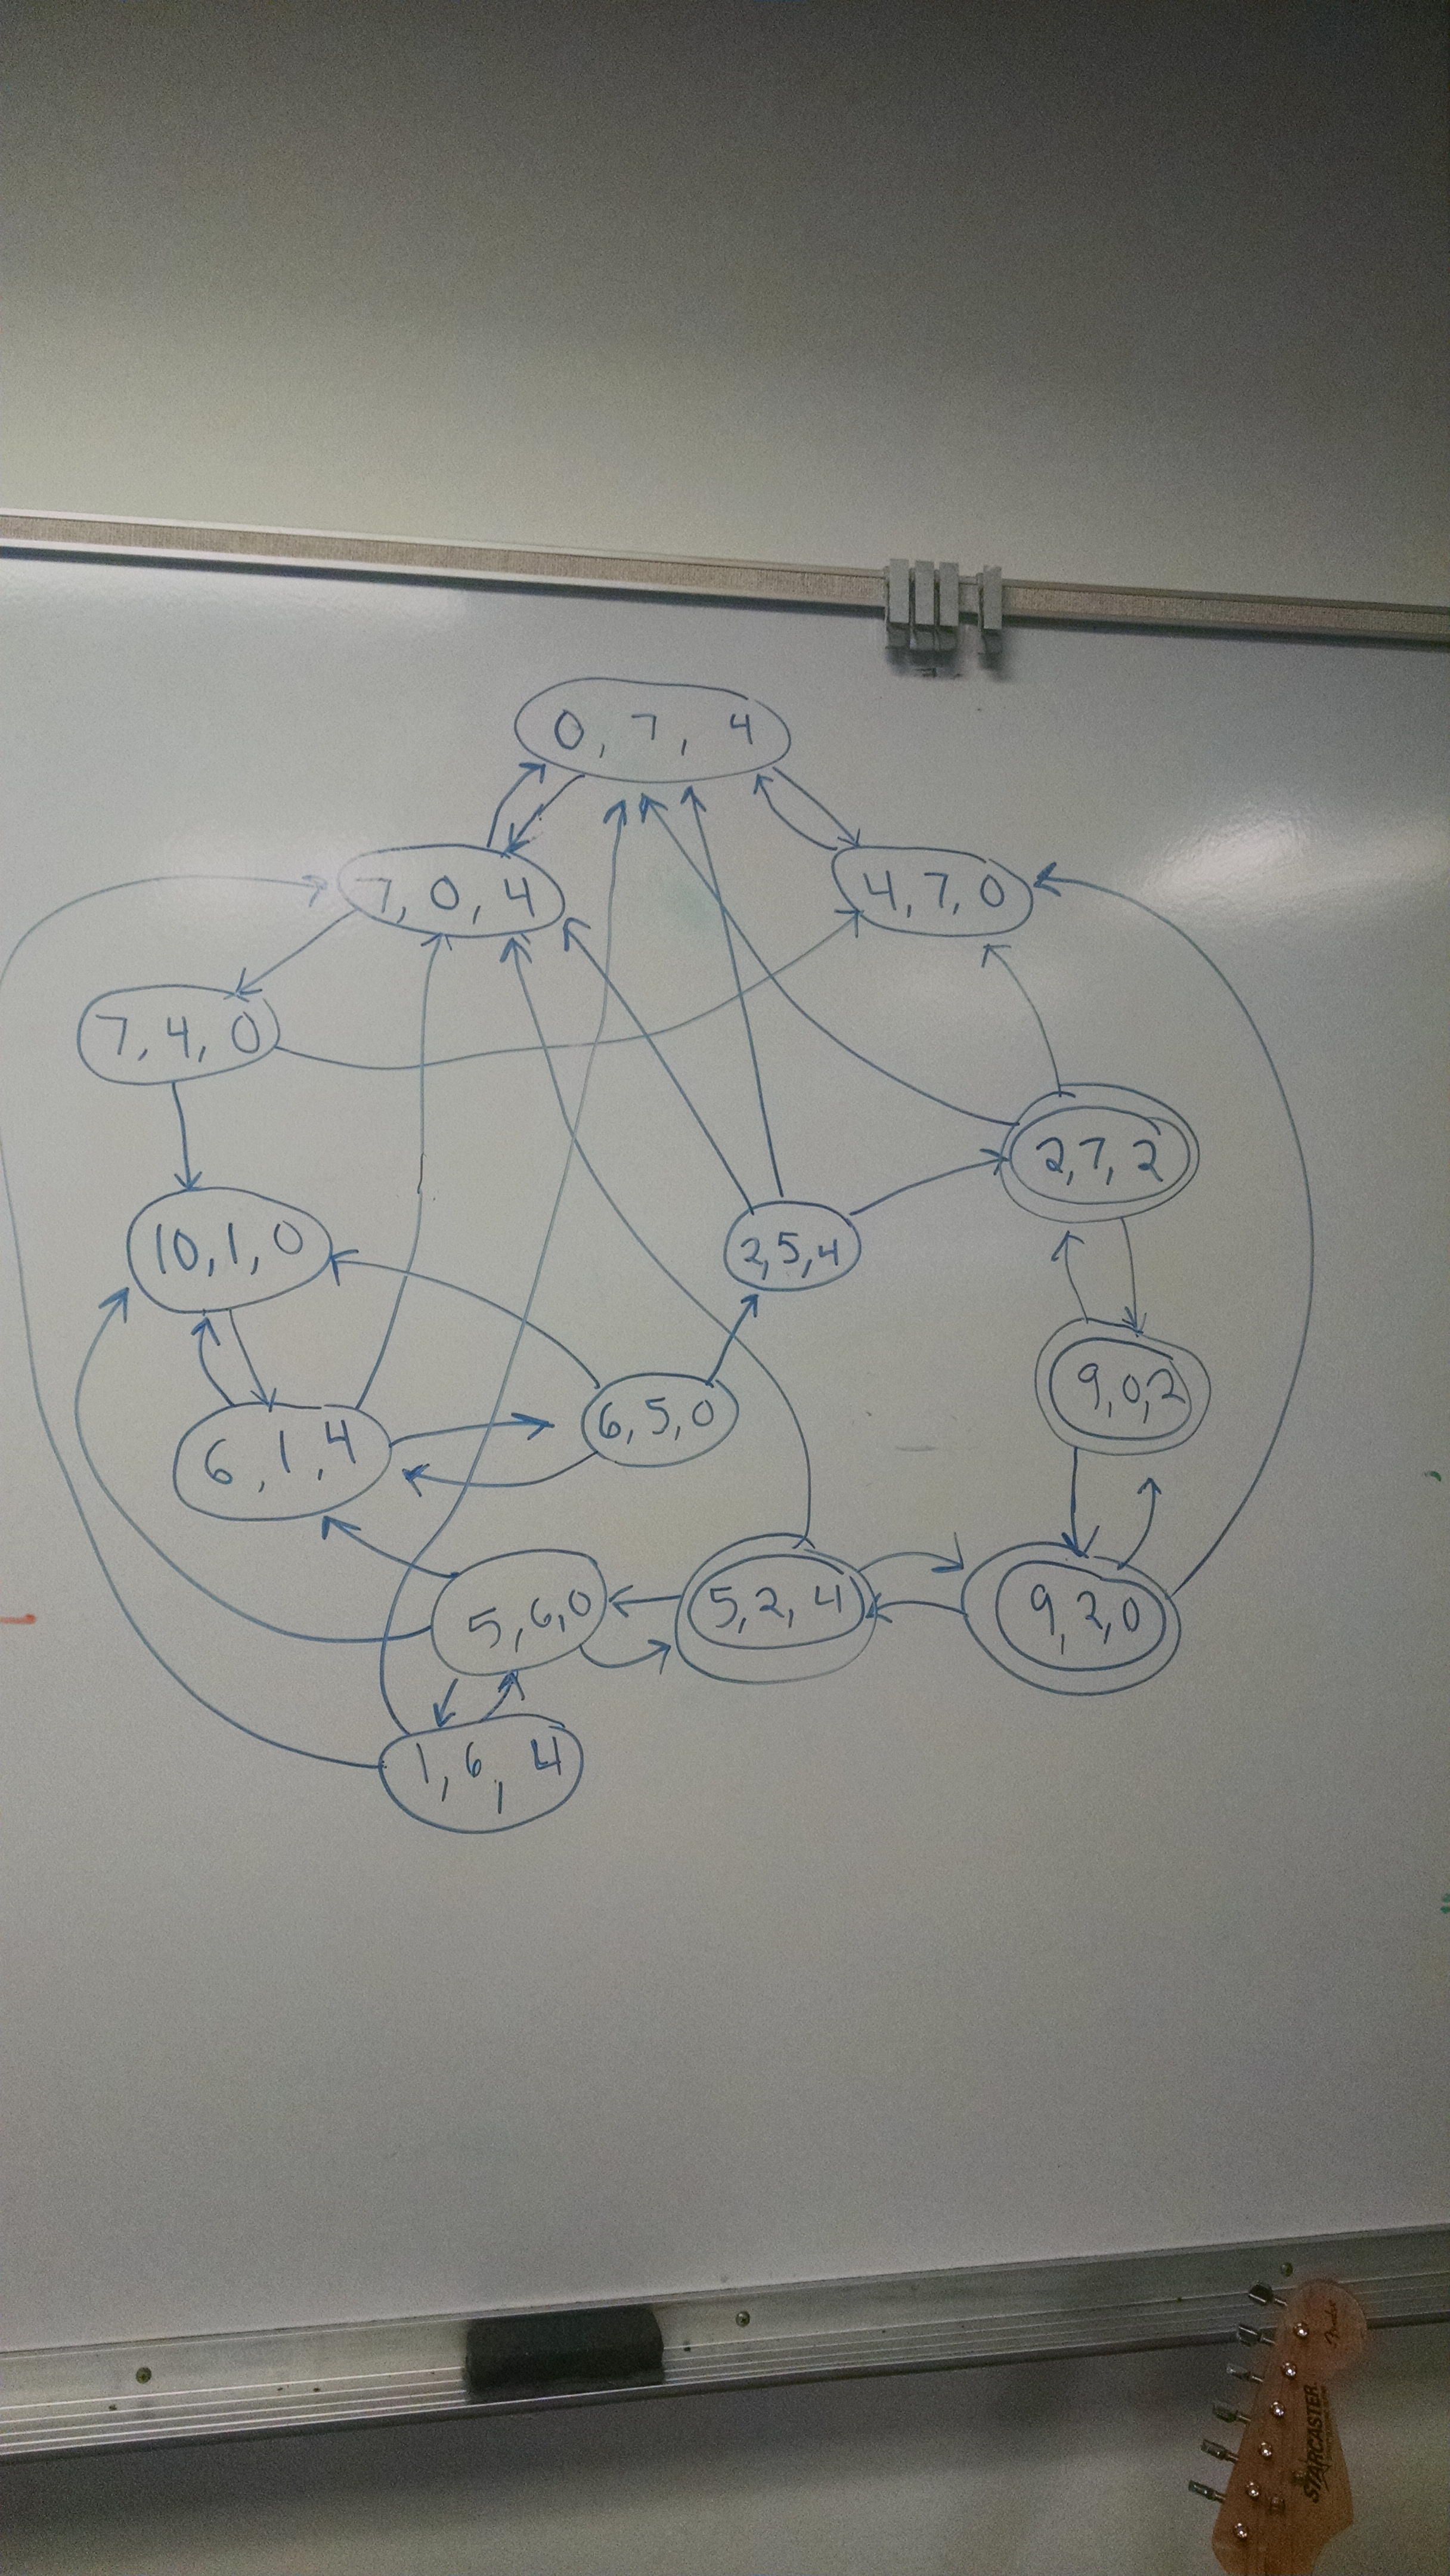
\includegraphics[width=0.5\textwidth]{graph.jpg}
\end{figure}

\begin{figure}[H]
\centering
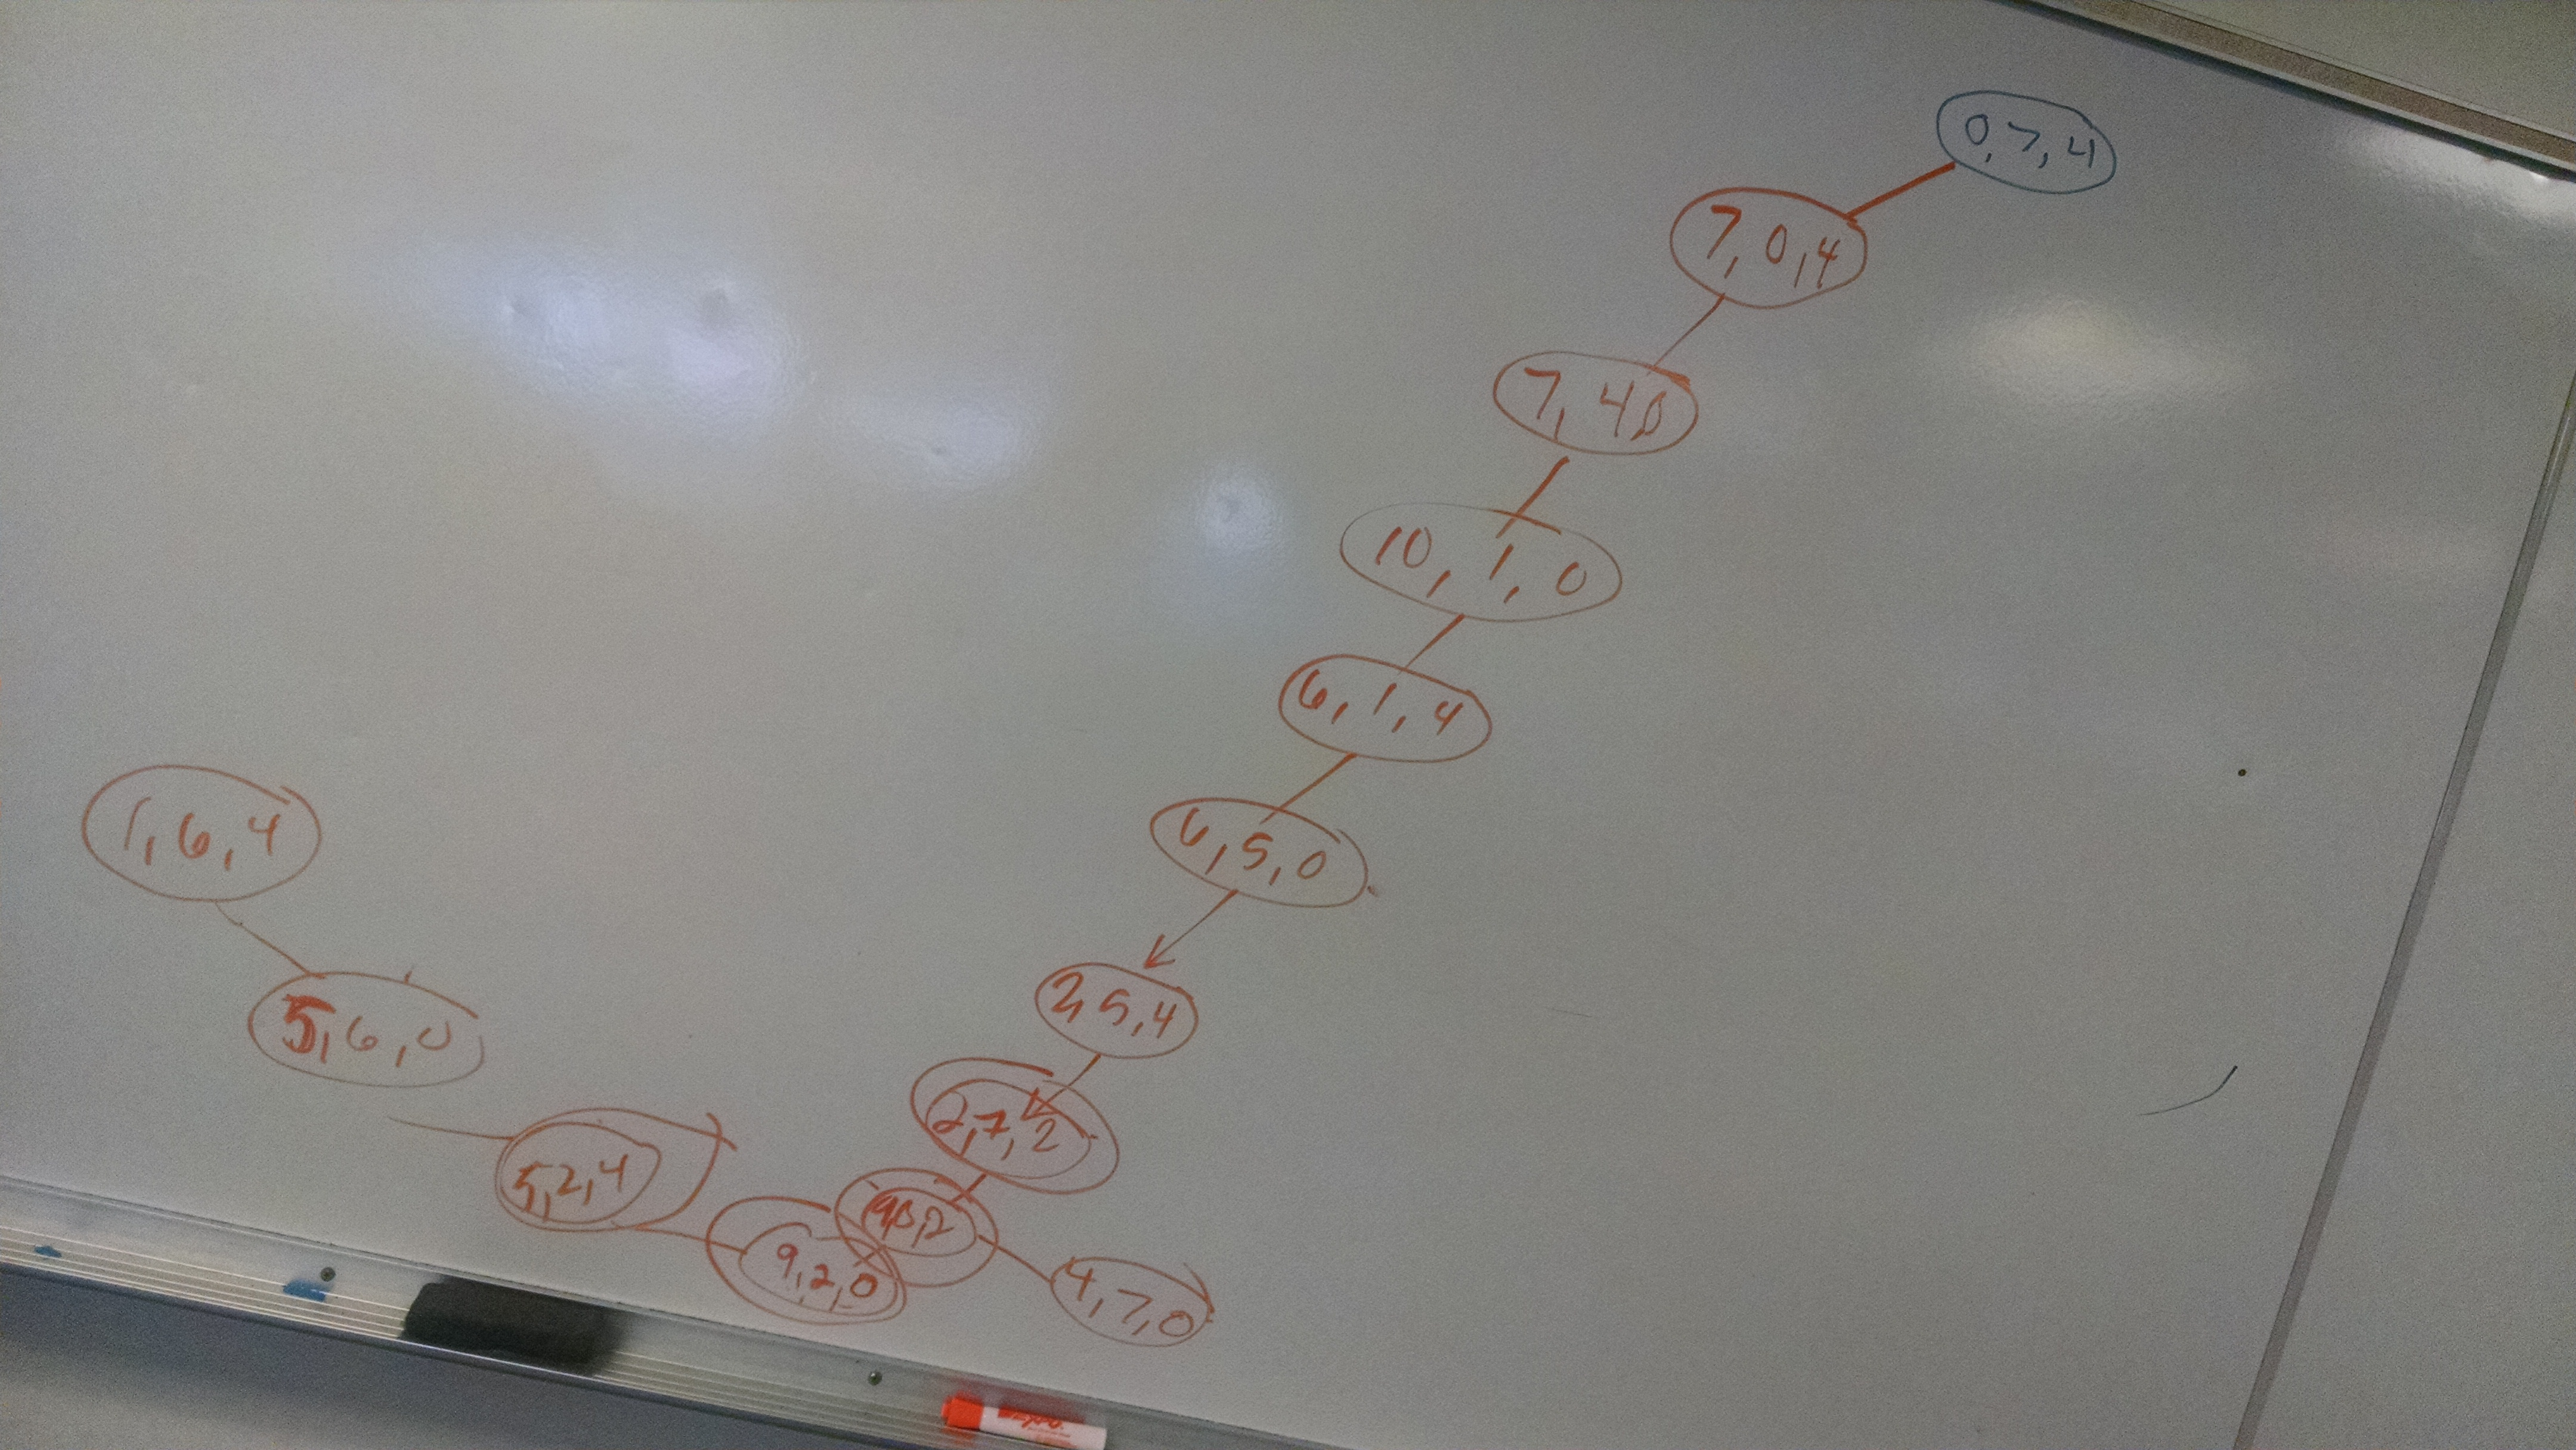
\includegraphics[width=0.5\textwidth]{spanningtree.jpg}
\end{figure}

a) The graphs we include show how to determine if there is a way to nodes given the specifications in the book from our starting point of (0,7,4). We did it using both breadth first search as well as depth first search. It is indeed possible and we have outlined all possible maneuvers we can do in our graphs. We determine every move based upon the next node we are moving to and the values for each node, comparing it at every step to the goal specifications from the problem that we wish to reach.

\end{document}
